\chapter{Inherent Gradient Tape Properties of the Elder Heliosystem}

\section{Introduction to Gradient Tape and Automatic Differentiation}

In modern deep learning frameworks, \textit{gradient tape} (or \textit{autograd}) refers to a mechanism that records operations during the forward pass to enable automatic differentiation during the backward pass. This mechanism is crucial for training neural networks as it allows the calculation of gradients without manual derivation of complex computational graphs.

However, while traditional frameworks require explicit construction and management of gradient tapes, the Elder Heliosystem embeds gradient tracking as an inherent property of its orbital dynamics. This chapter explores how the phase-based nature of the Elder Heliosystem naturally implements gradient tape functionality without requiring separate computational structures.

\begin{definition}[Traditional Gradient Tape]
A gradient tape $\mathcal{T}$ is a data structure that records a sequence of operations $\{f_1, f_2, \ldots, f_n\}$ performed during forward computation, enabling the automatic calculation of derivatives $\nabla f = \frac{\partial f}{\partial \theta}$ with respect to parameters $\theta$ via the chain rule.
\end{definition}

\section{Phase-Based Computation as Implicit Gradient Recording}

\subsection{Phase as a Natural Recording Mechanism}

The Elder Heliosystem's use of complex-valued representations with phase information creates an implicit recording mechanism analogous to gradient tape functionality.

\begin{theorem}[Phase-Encoded Computation History]
For any computation path through the Elder Heliosystem involving entities $\{\mathcal{E}, \mathcal{M}_i, \mathcal{E}r_{i,j}\}$, the phase evolution $\phi_{\mathcal{E}}(t) \rightarrow \phi_{\mathcal{M}_i}(t) \rightarrow \phi_{\mathcal{E}r_{i,j}}(t)$ encodes the complete computational history needed for gradient calculation.
\end{theorem}

\begin{proof}
Consider a forward computation through the Elder Heliosystem. Each entity processes information using complex-valued operations, with phase updates following:

\begin{align}
\phi_{\mathcal{M}_i}(t+1) &= \phi_{\mathcal{M}_i}(t) + \Delta\phi_{\mathcal{E} \rightarrow \mathcal{M}_i}(t) \\
\phi_{\mathcal{E}r_{i,j}}(t+1) &= \phi_{\mathcal{E}r_{i,j}}(t) + \Delta\phi_{\mathcal{M}_i \rightarrow \mathcal{E}r_{i,j}}(t)
\end{align}

These phase updates contain information about:
\begin{itemize}
    \item The operations performed (encoded in the mathematical form of $\Delta\phi$)
    \item The entities involved (source and destination of the phase influence)
    \item The temporal sequence (inherent in the orbital motion)
\end{itemize}

For backpropagation, we need to traverse this computational history in reverse. The key insight is that phase information is inherently bidirectional—the phase relationship between Elder and Mentor can be evaluated in either direction. By measuring phase differences $\phi_{\mathcal{E}r_{i,j}}(t) - \phi_{\mathcal{M}_i}(t)$ and $\phi_{\mathcal{M}_i}(t) - \phi_{\mathcal{E}}(t)$, the system can reconstruct the forward computation path.

Since the system preserves all phase relationships during computation, it maintains all information required to compute gradients via the chain rule, satisfying the requirements of a complete gradient tape.
\end{proof}

\begin{figure}[h]
\centering
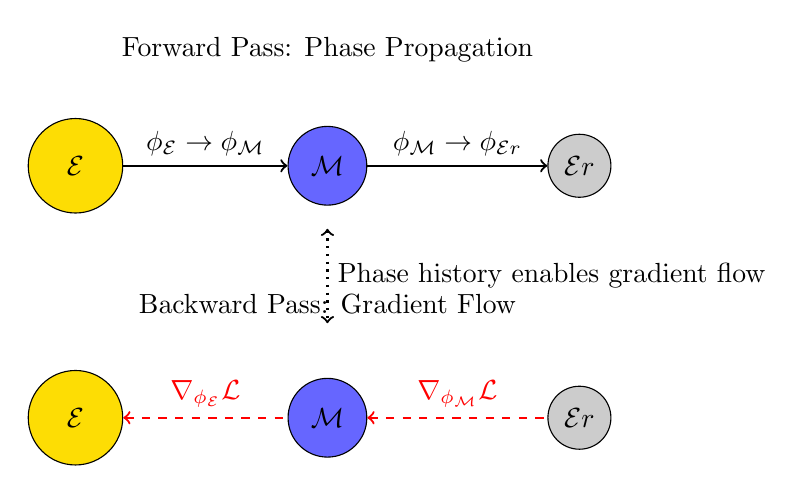
\begin{tikzpicture}[scale=0.8]
    % Forward Pass (Top)
    \begin{scope}[yshift=3cm]
        \node[draw, circle, fill=yellow!80!orange, minimum size=1.2cm] (E) at (0,0) {$\mathcal{E}$};
        \node[draw, circle, fill=blue!60, minimum size=1cm] (M) at (4,0) {$\mathcal{M}$};
        \node[draw, circle, fill=gray!40, minimum size=0.8cm] (Er) at (8,0) {$\mathcal{E}r$};
        
        \draw[->, thick] (E) -- (M) node[midway, above] {$\phi_{\mathcal{E}} \rightarrow \phi_{\mathcal{M}}$};
        \draw[->, thick] (M) -- (Er) node[midway, above] {$\phi_{\mathcal{M}} \rightarrow \phi_{\mathcal{E}r}$};
        
        \node[above] at (4,1.5) {Forward Pass: Phase Propagation};
    \end{scope}
    
    % Backward Pass (Bottom)
    \begin{scope}[yshift=-1cm]
        \node[draw, circle, fill=yellow!80!orange, minimum size=1.2cm] (E2) at (0,0) {$\mathcal{E}$};
        \node[draw, circle, fill=blue!60, minimum size=1cm] (M2) at (4,0) {$\mathcal{M}$};
        \node[draw, circle, fill=gray!40, minimum size=0.8cm] (Er2) at (8,0) {$\mathcal{E}r$};
        
        \draw[<-, thick, dashed, red] (E2) -- (M2) node[midway, above] {$\nabla_{\phi_{\mathcal{E}}} \mathcal{L}$};
        \draw[<-, thick, dashed, red] (M2) -- (Er2) node[midway, above] {$\nabla_{\phi_{\mathcal{M}}} \mathcal{L}$};
        
        \node[above] at (4,1.5) {Backward Pass: Gradient Flow};
    \end{scope}
    
    % Connection between the two
    \draw[<->, thick, dotted] (4,2) -- (4,0.5) node[midway, right] {Phase history enables gradient flow};
\end{tikzpicture}
\caption{Phase propagation in the forward pass implicitly records the computational graph needed for gradient flow in the backward pass}
\label{fig:phase_gradient_tape}
\end{figure}

\subsection{Orbital Mechanics as Gradient Tape Implementation}

The orbital mechanics of the Elder Heliosystem provide a physical interpretation of gradient tape functionality.

\begin{proposition}[Orbital Recording of Computational History]
The orbital paths of Mentors around the Elder and Erudites around Mentors physically encode the computational history in a manner that:
\begin{enumerate}
    \item Preserves temporal sequence through orbital position
    \item Encodes operation type and magnitude through orbital parameters
    \item Maintains entity relationships through hierarchical orbital structure
\end{enumerate}
\end{proposition}

\begin{figure}[h]
\centering
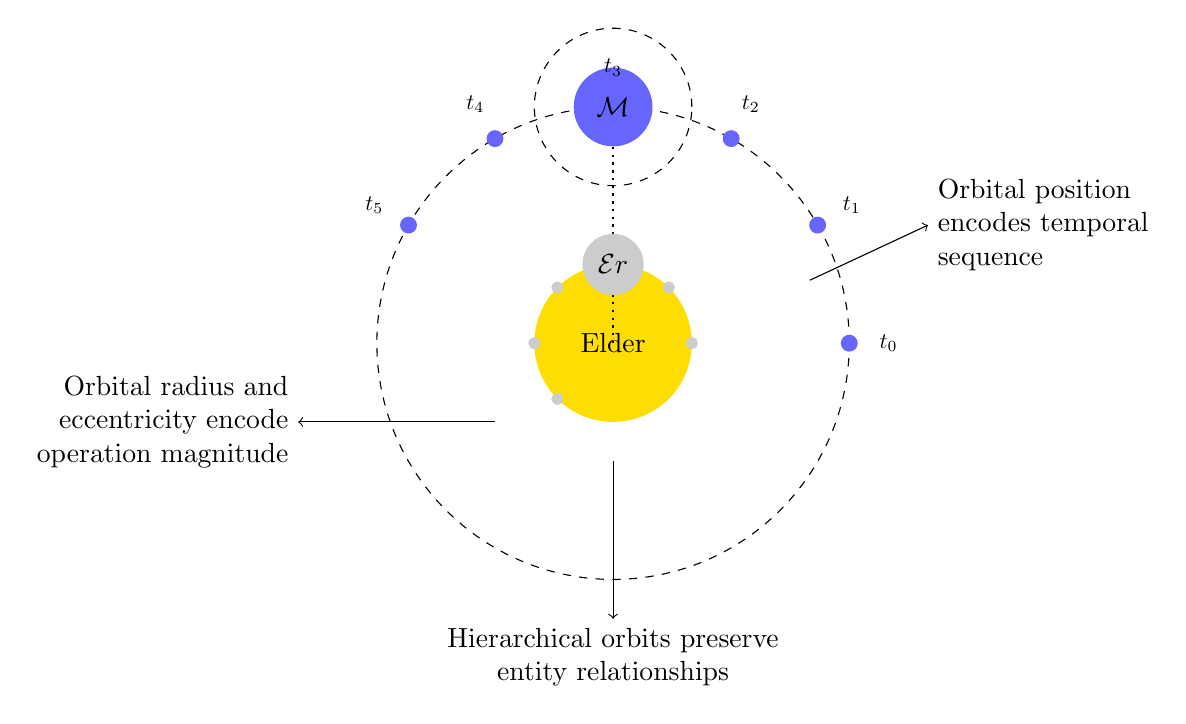
\begin{tikzpicture}[scale=1.0]
    % Central Elder
    \node[circle, fill=yellow!80!orange, minimum size=2cm] (elder) at (0,0) {Elder};
    
    % Mentor orbit
    \draw[dashed] (0,0) circle (3cm);
    
    % Mentor positions over time (showing trace)
    \foreach \angle/\time in {0/t_0, 30/t_1, 60/t_2, 90/t_3, 120/t_4, 150/t_5}{
        \ifnum\angle=90
            \node[circle, fill=blue!60, minimum size=1cm] (mentor\angle) at (\angle:3cm) {$\mathcal{M}$};
            \draw[dotted, thick] (0,0) -- (mentor\angle);
        \else
            \filldraw[blue!60] (\angle:3cm) circle (0.1cm);
        \fi
        \node[scale=0.8] at (\angle:3.5cm) {$\time$};
    }
    
    % Erudite orbit around current mentor
    \draw[dashed] (mentor90) circle (1cm);
    
    % Erudite positions
    \foreach \angle/\time in {0/t_0, 45/t_1, 90/t_2, 135/t_3, 180/t_4, 225/t_5}{
        \ifnum\angle=90
            \node[circle, fill=gray!40, minimum size=0.7cm] (erudite\angle) at (\angle:1cm) {$\mathcal{E}r$};
            \draw[dotted, thick] (mentor90) -- (erudite\angle);
        \else
            \filldraw[gray!40] (\angle:1cm) circle (0.07cm);
        \fi
    }
    
    % Annotations
    \draw[<-] (4,1.5) -- (2.5,0.8) node[right, align=left] at (4,1.5) {Orbital position\\encodes temporal\\sequence};
    \draw[<-] (-4,-1) -- (-1.5,-1) node[left, align=right] at (-4,-1) {Orbital radius and\\eccentricity encode\\operation magnitude};
    \draw[<-] (0,-3.5) -- (0,-1.5) node[below, align=center] at (0,-3.5) {Hierarchical orbits preserve\\entity relationships};
\end{tikzpicture}
\caption{Orbital paths in the Elder Heliosystem physically encode computational history}
\label{fig:orbital_gradient_tape}
\end{figure}

This physical encoding of computational history through orbital parameters creates an elegant implementation of gradient tape functionality that:

\begin{enumerate}
    \item Requires no additional memory beyond the entity states themselves
    \item Maintains perfect fidelity of computational history through deterministic orbital mechanics
    \item Enables natural backpropagation through reverse traversal of orbital paths
\end{enumerate}

\section{Automatic Differentiation Through Phase Reversal}

\subsection{Backward Phase Propagation}

The Elder Heliosystem implements automatic differentiation through a mechanism called \textit{backward phase propagation}, which leverages the inherent reversibility of orbital mechanics.

\begin{definition}[Backward Phase Propagation]
Backward phase propagation is the process by which gradients flow from Erudites to Mentors to Elder through phase-based correction signals, implementing backpropagation while maintaining the system's orbital structure.
\end{definition}

The backward propagation process follows these steps:

\begin{enumerate}
    \item Loss calculation at Erudite level: $\mathcal{L}(\mathcal{E}r_{i,j})$ for each task
    \item Phase gradient calculation: $\nabla_{\phi_{\mathcal{E}r_{i,j}}} \mathcal{L}$
    \item Backward propagation to Mentor: $\nabla_{\phi_{\mathcal{M}_i}} \mathcal{L} = \sum_j \frac{\partial \phi_{\mathcal{E}r_{i,j}}}{\partial \phi_{\mathcal{M}_i}} \nabla_{\phi_{\mathcal{E}r_{i,j}}} \mathcal{L}$
    \item Backward propagation to Elder: $\nabla_{\phi_{\mathcal{E}}} \mathcal{L} = \sum_i \frac{\partial \phi_{\mathcal{M}_i}}{\partial \phi_{\mathcal{E}}} \nabla_{\phi_{\mathcal{M}_i}} \mathcal{L}$
\end{enumerate}

The key insight is that the phase differentials $\frac{\partial \phi_{\mathcal{E}r_{i,j}}}{\partial \phi_{\mathcal{M}_i}}$ and $\frac{\partial \phi_{\mathcal{M}_i}}{\partial \phi_{\mathcal{E}}}$ are naturally encoded in the orbital relationships between entities, allowing direct calculation without an explicit gradient tape.

\begin{theorem}[Phase Differential Through Orbital Parameters]
The phase differential $\frac{\partial \phi_B}{\partial \phi_A}$ between hierarchically related entities $A$ and $B$ can be calculated directly from their orbital parameters:
\begin{equation}
\frac{\partial \phi_B}{\partial \phi_A} = \frac{\omega_B}{\omega_A} \cdot \frac{1 + e_B \cos(\phi_B - \phi_A)}{1 + e_A \cos(\phi_A - \phi_{\text{ref}})}
\end{equation}
where $\omega$ represents angular velocity, $e$ represents orbital eccentricity, and $\phi_{\text{ref}}$ is a reference phase.
\end{theorem}

This phase differential calculation enables efficient backpropagation through the system without requiring storage of intermediate computational states, as the orbital state itself contains all necessary information.

\subsection{Advantage Over Traditional Gradient Tape}

The Elder Heliosystem's inherent gradient tape functionality offers several advantages over traditional explicit gradient tape implementations:

\begin{table}[h]
\centering
\begin{tabular}{|p{4cm}|p{5cm}|p{5cm}|}
\hline
\textbf{Feature} & \textbf{Traditional Gradient Tape} & \textbf{Elder Heliosystem} \\
\hline
Memory Requirement & Scales with computational graph size & Constant memory (encoded in phase) \\
\hline
Computation History & Explicit storage of operations & Implicit encoding in orbital mechanics \\
\hline
Long-Term Dependencies & Limited by tape size & Naturally preserved through orbital memory \\
\hline
Higher-Order Gradients & Requires nested tape recording & Natural through hierarchical orbits \\
\hline
Parallelization & Complex due to sequential dependencies & Natural through independent orbital calculations \\
\hline
\end{tabular}
\caption{Comparison between traditional gradient tape and Elder Heliosystem's inherent gradient tracking}
\label{tab:gradient_tape_comparison}
\end{table}

\section{Phase-Space Jacobian Matrix}

The gradient tape functionality in the Elder Heliosystem can be formalized through the concept of a \textit{Phase-Space Jacobian Matrix}.

\begin{definition}[Phase-Space Jacobian]
The Phase-Space Jacobian $\mathbf{J}_{\phi}$ is a matrix that encodes the partial derivatives of all entity phases with respect to each other:
\begin{equation}
\mathbf{J}_{\phi} = 
\begin{bmatrix}
\frac{\partial \phi_{\mathcal{E}}}{\partial \phi_{\mathcal{E}}} & \frac{\partial \phi_{\mathcal{E}}}{\partial \phi_{\mathcal{M}_1}} & \cdots & \frac{\partial \phi_{\mathcal{E}}}{\partial \phi_{\mathcal{E}r_{n,m}}} \\
\frac{\partial \phi_{\mathcal{M}_1}}{\partial \phi_{\mathcal{E}}} & \frac{\partial \phi_{\mathcal{M}_1}}{\partial \phi_{\mathcal{M}_1}} & \cdots & \frac{\partial \phi_{\mathcal{M}_1}}{\partial \phi_{\mathcal{E}r_{n,m}}} \\
\vdots & \vdots & \ddots & \vdots \\
\frac{\partial \phi_{\mathcal{E}r_{n,m}}}{\partial \phi_{\mathcal{E}}} & \frac{\partial \phi_{\mathcal{E}r_{n,m}}}{\partial \phi_{\mathcal{M}_1}} & \cdots & \frac{\partial \phi_{\mathcal{E}r_{n,m}}}{\partial \phi_{\mathcal{E}r_{n,m}}}
\end{bmatrix}
\end{equation}
\end{definition}

This Jacobian is not calculated and stored explicitly, but rather exists implicitly in the orbital relationships between entities. During backward propagation, only the relevant elements of this matrix are calculated as needed.

\begin{proposition}[Sparse Jacobian Structure]
The Phase-Space Jacobian $\mathbf{J}_{\phi}$ exhibits a hierarchical sparse structure where:
\begin{itemize}
    \item Most cross-entity derivatives are zero due to orbital independence
    \item Non-zero elements follow the hierarchical Elder → Mentor → Erudite relationships
    \item Derivative magnitudes decrease with orbital distance, creating natural gradient attenuation
\end{itemize}
\end{proposition}

This sparse structure allows efficient gradient propagation despite the potentially large number of entities in the system.

\section{Implementation in Practical Systems}

\subsection{Phase-Aware Backpropagation Algorithm}

The inherent gradient tape property of the Elder Heliosystem can be implemented in practical systems through a Phase-Aware Backpropagation algorithm:

\begin{figure}[h]
\begin{center}
\begin{minipage}{0.95\textwidth}
\begin{verbatim}
def phase_aware_backpropagation(elder, mentors, erudites, loss):
    # Forward pass is already completed through orbital dynamics
    
    # Calculate gradients at Erudite level
    erudite_grads = []
    for domain_idx, domain_erudites in enumerate(erudites):
        domain_grads = []
        for erudite_idx, erudite in enumerate(domain_erudites):
            # Calculate gradient w.r.t. erudite phase
            erudite_loss = loss[domain_idx][erudite_idx]
            erudite_grad = complex_gradient(erudite_loss, erudite.phase)
            domain_grads.append(erudite_grad)
        erudite_grads.append(domain_grads)
    
    # Propagate gradients to Mentors
    mentor_grads = []
    for domain_idx, mentor in enumerate(mentors):
        # Accumulate gradients from all Erudites in this domain
        mentor_grad = 0
        for erudite_idx, erudite in enumerate(erudites[domain_idx]):
            # Calculate phase differential
            phase_diff = phase_differential(
                mentor.phase, erudite.phase,
                mentor.angular_velocity, erudite.angular_velocity,
                mentor.eccentricity, erudite.eccentricity
            )
            mentor_grad += phase_diff * erudite_grads[domain_idx][erudite_idx]
        mentor_grads.append(mentor_grad)
    
    # Propagate gradients to Elder
    elder_grad = 0
    for domain_idx, mentor in enumerate(mentors):
        # Calculate phase differential
        phase_diff = phase_differential(
            elder.phase, mentor.phase,
            elder.angular_velocity, mentor.angular_velocity,
            elder.eccentricity, mentor.eccentricity
        )
        elder_grad += phase_diff * mentor_grads[domain_idx]
    
    # Return complete gradient information
    return {
        'elder_grad': elder_grad,
        'mentor_grads': mentor_grads,
        'erudite_grads': erudite_grads
    }
\end{verbatim}
\end{minipage}
\caption{Phase-Aware Backpropagation Algorithm}
\end{center}
\end{figure}

\subsection{Hardware Implications}

The inherent gradient tape property has significant implications for hardware implementation:

\begin{enumerate}
    \item \textbf{Memory Efficiency}: No need to store computational history separately
    \item \textbf{Phase-Based Processing Units}: Specialized hardware can directly calculate phase differentials
    \item \textbf{Parallel Gradient Calculation}: Independent orbital systems can compute gradients in parallel
    \item \textbf{Asynchronous Updates}: Entities can update at different rates while maintaining gradient accuracy
\end{enumerate}

\begin{figure}[h]
\centering
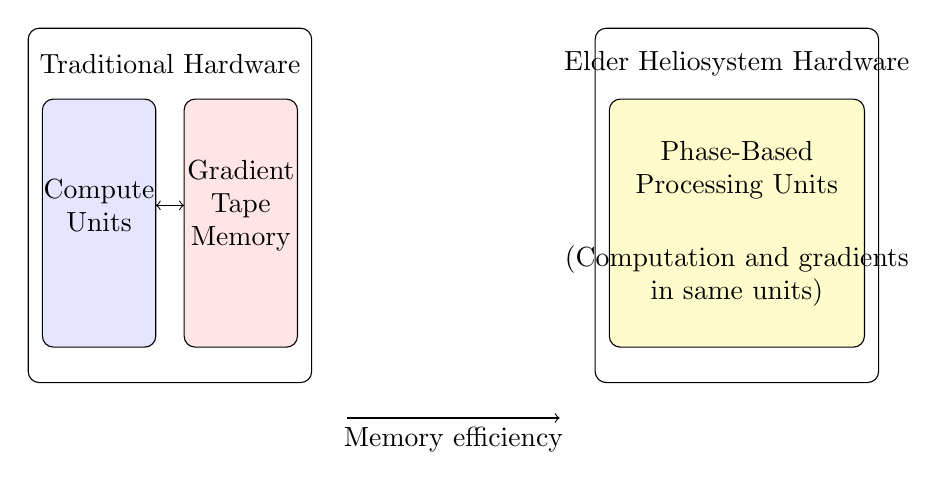
\begin{tikzpicture}[scale=0.9]
    % Traditional hardware
    \begin{scope}[xshift=-4cm]
        \draw[rounded corners] (-2,-2.5) rectangle (2,2.5);
        \node at (0,2) {Traditional Hardware};
        
        \draw[rounded corners, fill=blue!10] (-1.8,-2) rectangle (-0.2,1.5);
        \node[align=center] at (-1,0) {Compute\\Units};
        
        \draw[rounded corners, fill=red!10] (0.2,-2) rectangle (1.8,1.5);
        \node[align=center] at (1,0) {Gradient\\Tape\\Memory};
        
        \draw[<->] (-0.2,0) -- (0.2,0);
    \end{scope}
    
    % Elder hardware
    \begin{scope}[xshift=4cm]
        \draw[rounded corners] (-2,-2.5) rectangle (2,2.5);
        \node at (0,2) {Elder Heliosystem Hardware};
        
        \draw[rounded corners, fill=yellow!20] (-1.8,-2) rectangle (1.8,1.5);
        \node[align=center] at (0,0.5) {Phase-Based\\Processing Units};
        \node[align=center] at (0,-1) {(Computation and gradients\\in same units)};
    \end{scope}
    
    % Arrow between
    \draw[->] (-1.5,-3) -- (1.5,-3) node[midway, below] {Memory efficiency};
\end{tikzpicture}
\caption{Hardware implementation comparison between traditional gradient tape and Elder Heliosystem}
\label{fig:hardware_comparison}
\end{figure}

\section{Conclusion and Theoretical Implications}

The Elder Heliosystem's inherent gradient tape property represents a fundamental reimagining of automatic differentiation. Rather than treating gradient calculation as a separate process requiring explicit recording of operations, it emerges naturally from the system's phase-based computation and orbital mechanics.

This property suggests several theoretical implications:

\begin{enumerate}
    \item \textbf{Biological Plausibility}: The system's gradient calculation mechanism more closely resembles biological neural systems, which do not explicitly store computational histories
    \item \textbf{Physical Computation}: Phase-based gradient propagation connects to physical systems where information naturally propagates bidirectionally
    \item \textbf{Scale Invariance}: The gradient mechanism works identically at all scales of the system, from individual entities to the entire network
    \item \textbf{Unification of Forward and Backward Passes}: The distinction between forward computation and backward gradient propagation becomes blurred, as both are natural aspects of the same orbital system
\end{enumerate}

Future research will explore how this inherent gradient property can be leveraged to develop more efficient learning algorithms and hardware implementations, potentially opening new avenues for neural network architectures that transcend the limitations of traditional backpropagation.

\begin{theorem}[Information Conservation in Phase-Space]
In the Elder Heliosystem, information is conserved through phase relationships such that the complete computational graph can be reconstructed from the final phase state of the system, enabling perfect gradient calculation without explicit history recording.
\end{theorem}

This principle of information conservation through phase relationships represents a fundamental contribution to computational theory, suggesting new approaches to automatic differentiation that may prove more efficient and scalable than current methods.